\chapter{Background \& Objectives}
\vspace{-20pt}
%This section should discuss your preparation for the project, including background reading, your analysis of the problem and the process or method you have followed to help structure your work.  It is likely that you will reuse part of your outline project specification, but at this point in the project you should have more to talk about. 

%\textbf{Note}: 

%\begin{itemize}
%   \item All of the sections and text in this example are for illustration purposes. The main Chapters are a good starting point, but the content and actual sections that you include are likely to be different.
   
%   \item Look at the document on the Structure of the Final Report for additional guidance. 
   
%\end {itemize}
\section{Background \& Analysis}
%What was your background preparation for the project? What similar systems did you assess? What was your motivation and interest in this project? 

%  BACKGROUND
%    - Checked out drones, how they fly in general and what kind of things is possible.
%    - Checked out specifically the AR Drone 2.0 +  it's capabilities
%      - How to control it?
%        -ROS, the C library it was provided with, .js nodes, CVDrone.
%    -Vision stuff
%      - Monocular vision for object detection
%      - Using a single camera for determining depth of objects (Not totally necessary for me, unknown at the time)
%    - Other projects with the AR Drone.
%

\subsection{Drone capabilities}
The platform for this project was the Parrot AR.Drone 2.0, which is a quad-copter with limited sensor capabilities. Before this project could be pursued these capabilities had to be fully assessed to understand the limits of the quad-copter, ensure the project was possible and to limit the scope of the project.


\subsubsection{Cameras}
The first camera is a high quality front-facing camera, traditionally used to take pictures or help a user guide the quad-copter when it isn't in line of sight. The front facing camera has a maximum 720p resolution with a 30fps frame rate and a 92$^{\circ}$ viewing angle. In a vision based navigation system this would be the camera in use, as it has the best view of potential collisions and objects in the path of the drone. It also has a higher resolution, which will improve our features but also increase computation time although the effects of the increased computation is likely to be negligible.

The second camera is a downward facing camera which is mainly used to calculate ground speed within the drone but it can be used to take pictures by the user. This second camera is a Quarter Video Graphics Array with a resolution of 320 x 240.  While this camera would not be able to be used in a navigation system due to it's orientation, it could be used in other vision projects such as mapping from above or navigating using pre-planned flight instructions from signs on the floor.


\subsubsection{Processor + RAM}
The on-board processor of the AR Drone 2.0 is a 1GHz 32 bit ARM Cortex A8 processor. This processor is not available to the user without altering the firmware that is directly on the drone. If this route were to be followed, a lot of safety features would have to be re-written, along with software to directly control the motors in the drone and software to accept commands from elsewhere. This would be out of scope for a project of this size, so the best alternate solution is to perform processing elsewhere. Due to the higher processing power available elsewhere, this is likely more beneficial for a vision based system.


\subsubsection{Connectivity}
In order to connect to the quad-copter from a separate device, the drone has a wireless access point. This wireless access card allows for connection to B/G and N connections, meaning it can go up to 100Mb/s \cite{Nstandard} Connection speed however could be an issue, slowing down transmission of images from the drone and commands to the drone.

 To properly assess this potential bottleneck, the time taken to transfer 100 packets of information to the drone and back was taken and averaged via the "ping" command in a terminal when connected to the drone. This connection speed average is shown in figure 1, the outliers are likely to produce freezes within the program and vision calculations, so some robustness in our implementation will be needed to deal with this.

\begin{figure}
\centering
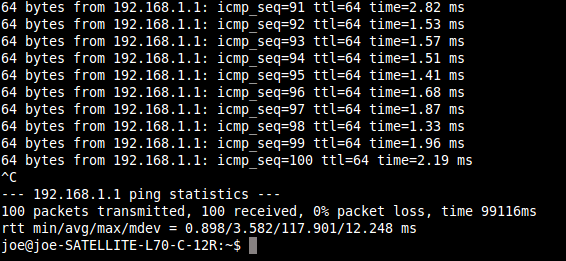
\includegraphics[scale=0.5]{PingScreen.png}
\caption{The results of the ping command when connected to the AR Drone 2.0}
\end{figure}
\subsubsection{Other sensors}
\begin{itemize}
  \item 3 axis gyroscope 2000°/second precision
  \item 3 axis accelerometer +-50mg precision
  \item 3 axis magnetometer 6° precision
  \item Pressure sensor +/- 10 Pa precision
  \item Ultrasound sensors for ground altitude measurement
\end{itemize}


\subsection{Drone control}
Being able to control the drone is another important aspect of this project, as the project is not possible without at least access to the camera feeds. There are a couple of important factors that needed to be considered for this part of the background research such as language, ease of use, ease of implementation, feature availability and licenses.


\subsubsection{AR Drone SDK}
This is the Source Development Kit provided by the developers of the AR Drone 2.0\cite{DroneAPI}, provided in C with extensive documentation\cite{DroneDevGuide}. This, however, is very confusing to read and made it quite difficult to follow and implement. Coupled with inexperience with C, drones and computer vision, the project would have been made much harder using this software to control the drone. The SDK is provided under Parrot's own license, included in Appendix A.


\subsubsection{Node Copter}
This is a JavaScript based control software, provided here\cite{nodecop}. Having used Java before, JavaScript would be easier to learn quickly. There are also libraries available to perform computer vision however they seemed to be inconsistent with their features, as I was unable to find a full implementation of OpenCV. Not knowing the exact algorithms that were going to be used for the vision meant this wasn't an option at the time.


\subsubsection{Robot Operating System Driver}
ROS is a collection of frameworks provided for use with Robotics, in this case a driver provided for the AR Drone 2.0\cite{ROSDrone}. The full extent of the capabilities of the driver are unknown to me, as learning ROS would have been very time consuming in this time constrained project and I decided not to continue this line of investigation.


\subsubsection{CVDrone}

CVDrone is software that combines control of the AR Drone 2.0 with OpenCV, an open source computer vision library\cite{CVDrone}. This software provides an API for C++, with easy to read documentation and example code. It's distributed under the GNU Lesser General Public License\cite{GNULGPL} and was the final choice for controlling the drone.  This was an easy choice, as it already contained the full OpenCV vision library as well as providing an easy to understand and learn method of implementation.

CVDrone acts as middleware between the project I am creating and the drone, giving me access to an API that allows for simple commands to be sent such as "takeOff()", "landing()" and "move3d(x, y, z, r)". This makes moving the drone a much easier task, simplifying what could have been an entire project itself into a few API calls. This software also provides access to OpenCV libraries by default, this isn't necessary and includes parts of OpenCV we won't need but does save time in implementing them as separate libraries.

Another small benefit of CVDrone is that it fixes an orientation issue within the original SDK for the AR Drone, flipping the Z axis so that as the value increases the drone flies up rather than down. This is a minor issue but it does avoid some confusing Z values.

\subsection{Vision}
While familiar with theory, implementation and more complicated theory had to be researched to gain a fuller understanding of what is possible within a moving, monocular system.


\subsubsection{Monocular vision}
One of the main issues facing a vision based obstacle avoidance system is a lack of depth inherent in a single camera system. Depth perception from a single camera is a difficult problem, as depth is usually determined through the calculation of disparity between two images of the same area from a slightly different perspective \cite{StereoDepth}. However this becomes less of an issue within a moving system and a monocular system can even be used for 3D mapping of objects using optical flow\cite{3DMapOpFlowMono} in this case.

This indicates to me that it's possible to implement a system that will provide sufficient obstacle avoidance ability within the drone.

\subsubsection{Monocular obstacle avoidance}
Further research into monocular obstacle avoidance found papers referencing how optical flow is used biologically in flying insects\cite{citeulike:9515178} and birds\cite{opticalFlowBirds}. This gave me the idea of using the phenomenon of relative motion to avoid obstacles that are closer to the camera and led to research further in the direction of using optical flow rather than depth mapping.

 In the search for optical flow based obstacle avoidance, the papers \cite{souhila2007optical} and \cite{PhoneObstacleAvoidance} seemed relevant in achieving the projects goals. \cite{PhoneObstacleAvoidance} was closer to the original intent in using optical flow and final goal of the project and as such became the basis for this project.
 
 The paper describes a method of finding, classifying and then warning about objects within a moving monocular system using computer vision. For this project however, we only needed to be able to identify and avoid objects within the drones view. \S3.1 of the paper details 7 steps to identify obstacles in the path of the camera and whether or not they should be avoided. A summary of these 7 steps is shown below:
\begin{description}
	\item [Step 1 - Interest Point Extraction] In this step, features are detected and turned into interest points. In the paper, the interest points are detected using a grid sampling method in order to allow for equal spread of features throughout the image. This means that less textured regions of the image still factor in to steps further down the line.
	
	\item[Step 2 - Interest Point Tracking] Here, the interest points from step 1 are taken and the Lucas-Kanade \cite{Lucas_KanadeOF} optical flow algorithm is applied to track them through multiple frames. Motion vectors, magnitude and angle of motion are all calculated within this step as well, which will be used later.
	
	\item[Step 3 - Camera/Background motion estimation] Now that interest points are being tracked, background motion/camera motion is estimated.
	
	This is done by generating a 3 x 3 homography using a robust RANSAC method and then multiplying this homography by the original points in order to produce an estimate position of the point in the next frame. The estimated point position is then compared to the actual point position, if the estimation error is larger than a particular threshold then the point is considered foreground.
	
	\item[Step 4 - Motion Classes estimation] These foreground points are then clustered together based using a hierarchical agglomerative technique on their motion magnitude and angular deviation from each cluster centroid. This is done in 2 phases. 
	
	The first phase sorts the interest points in descending order based on the number of occurrences of their motion vector angle. Then a new cluster is formed using the first interest point's motion vector angle as it's centroid.
	
	The second phase then calculates the remaining interest points motion magnitude and angular deviation from the cluster centroid. If the motion magnitude is equal to the centroid point and the angular deviation is beyond a certain threshold, the next interest point is added to that cluster. Otherwise, that interest point becomes the centroid for a new cluster. This is applied recursively until all points are part of a cluster.
	
	\item[Step 5 - Refinement of clusters/Interest Point refinement] Once the points are clustered, they're refined by applying a k-Nearest Neighbours algorithm. Each point is clustered again using k-NN with the Euclidean distance, if at least half of it's nearest neighbours do not belong to the same motion class, the point is removed from the cluster.
	
	\item[Step 6 - Motion Classes' temporal consistency] Now the clusters are refined, we memorise their trajectory over the past few frames and predict the position of the cluster. This is in order to protect clusters against partial occlusion, noise and image distortion.
	
	\item[Step 7 - Obstacle relevance establishing] Finally, the objects nature relevant to the camera is established. If the object is moving towards the cameras focus point, it is classed as {\em approaching}, otherwise it is classed as {\em departing}. Then a polar grid is projected onto the image and if the object is within a certain range, it is classed as {\em urgent}. Otherwise, the object will be classified as {\em normal}.
\end{description}

%i.e  dense interest points, fuzzyRansac, Multiple view geometry, agglomerative heirarchichal clustering, polar grids + focal points of cameras.
\subsubsection{Further reading}
This paper also introduced multiple concepts that needed further research to gain a proper understanding of the methods employed by the paper. These new concepts were Grid sampling of dense interest points, homography generation using RANSAC, polar grids and calculating the focal point of a camera.

\begin{description}
	\item [Grid sampling of dense interest points] For research on this topic, the paper "Dense Interest Points"\cite{DenseInterest} was a great help, providing an insight to the idea of sampling many interest points from an image. OpenCV does allow for multiple methods of extracting features and some of these techniques are classified as "Dense" techniques.]
	
	\item [Homography generation] The paper required the use of homographies to predict future locations of points and it did so through the use of a method called fuzzy RANSAC. A homography is generally kept in the form of a matrix and is used to relate 2 images from the same camera that have been taken from a different angle. This can be done using a regular RANSAC method, however in our paper it's done with a more robust version.
	
	\item[Fuzzy RANSAC] This is a method of implementing RANSAC that uses fuzzy logic to help classify the sample set into 3 sets: Good, vague and bad. RANSAC is then only applied only to the good sample set, which improves the robustness of the algorithm.

\end{description}

\subsubsection{OpenCV}
Having never used OpenCV one of the main background research points was learning how to use and implement OpenCV into my own applications. As part of this research I looked at example code provided with OpenCV and developed some simple implementations of basic vision on camera feeds to be certain I understood how to use the libraries correctly.

This also allowed for further understanding of OpenCV's data types that are used such as cv::Mat and cv::Point2f, Matrixes and float 2D Points respectively, as well as a little practice with C++ before the main project.

The choice to use OpenCV is a clear one, as it's one of the largest, fully featured computer vision libraries available and is provided fully for the C++ language. The open source nature of OpenCV also helps improve understanding of what's happening behind the scenes, which will potentially help improve the time frame of understanding OpenCV for the project. OpenCV is also extensively documented and has a large number of users, meaning that problems will be quicker to solve than if a more obscure library were being used.

\subsection{Tasks to be undertaken and where they came from}

The paper \cite{PhoneObstacleAvoidance} breaks down the overall structure of this problem quite well, making most of the visions steps into specific tasks. It doesn't cover the entire project however, as adaptations needed to be made to get the vision to interact with the drone as well as a drone controller. 

This essentially means that there are 2 major parts to this project, Vision and Drone control.

\subsubsection{Vision}
The paper splits the vision into 7 steps, so initially these 7 steps were used as tasks to be completed, however they were too large to be considered stories in my methodology. In order to help fit them into my methodology, I considered most steps an "Epic", consisting of multiple stories. The only exception to this was the feature detection, feature tracking through frames and interest point refinement, as these steps were small enough to be considered stories of their own right. A break down of each epic follows:

\begin{description}
	\item[Epic 1 : Camera/background motion estimation] Step 3 of 7.\\
	\vspace{-15pt}
	\begin{itemize}
		\item Homography generation
		\item Prediction of point placement in future frames
		\item Classify points based on estimation error
	\end{itemize}
	\item[Epic 2 : Motion Classes estimation] Step 4 of 7.\\
	\vspace{-15pt}
	\begin{itemize}
		\item Sort motion vectors in descending order based on number of occurences
		\item Classify each point using agglomerative hierarchical clustering
	\end{itemize}
	\item[Epic 3 : Motion classes' temporal consistency] Step 6 of 7.\\
	\vspace{-15pt}
	\begin{itemize}
		\item Store motion class centroids trajectory over N past frames.
		\item Predict position of the object compensated with camera/background motion.
	\end{itemize}
	\clearpage
	\item[Epic 4 : Relevance establishing] Step 7 of 7.\\
	\vspace{-15pt}
	\begin{itemize}
		\item Find cameras focal point
		\item Classify objects as approaching or departing based on the trajectory of the motion class
		\item Implement a polar grid projection
		\item Classify objects as Urgent or Normal, based on distance from drone.
	\end{itemize}
\end{description}

\subsubsection{Drone control}
This section is the part of the project that relates to controlling the drone and tying it in to the vision system above. While the vision system is considered a collection of Epics, the drone controller can be considered an Epic in itself, as it's not the main component of this project. The drone controller acts as a method of implementing the vision into a robotics system, rather than being a main focus of work.

\begin{description}
	\item[PID controller] Here we implement a PID controller, which will be the main part of the controller, allowing for 
	\item[API for drone control] This story is all about implementing a method of communicating direction to the drone, as CVDrone only provides move3d(x, y, z, r) where x, y, z and r are velocities. 
\end{description}
%\section{Analysis}
%Taking into account the problem and what you learned from the background work, what was your analysis of the problem? How did your analysis help to decompose the problem into the main tasks that you would undertake? Were there alternative approaches? Why did you choose one approach compared to the alternatives? 

%There should be a clear statement of the objectives of the work, which you will evaluate at the end of the work. 

%In most cases, the agreed objectives or requirements will be the result of a compromise between what would ideally have been produced and what was felt to be possible in the time available. A discussion of the process of arriving at the final list is usually appropriate.

%i.e explain our process (personal kanban/scrum)
\clearpage
\section{Process}
%You need to describe briefly the life cycle model or research method that you used. You do not need to write about all of the different process models that you are aware of. Focus on the process model that you have used. It is possible that you needed to adapt an existing process model to suit your project; clearly identify what you used and how you adapted it for your needs.
%==============================================================================

%==============================================================================
For this project, a methodology was followed in order to keep the project on track and keep forward progress. Here I will introduce the initial methodology, explaining the thoughts behind any decisions and any artifacts that will be produced. After the initial methodology, the changes that took place throughout the experience are detailed along with the reasoning and perceived effects on the work flow.

The initial methodology draws mainly from scrum\cite{PersonalScrum} and kanban\cite{PersonalKanban}, taking an iterative approach to development and process improvement from scrum and using a kanban workflow for use throughout the sprints.\\

Sprints are used so that constant improvement can be made to the process without interrupting potential works in progress and the kanban system is used during the sprint to ensure work is done effectively and progress within the project is measurable. It also forces a limit on work done, quantization of goals and combined with sprints, ensures goals are small enough to be achievable within the sprint time frame.
\subsection{Initial methodology and artefacts}
%==============================================================================
\begin{description}
	\item[Sprints]
	Each development iteration will take place in a sprint, with each sprint lasting 2 weeks. During this time, a particular number of stories should be completed from the sprint backlog and if they're not, they're added back onto the project backlog.\\
	
	The 2 week sprint will allow for supervisory meetings at the end and beginning of a sprint, as well as a mid-sprint meeting. At the beginning of the sprint, the meeting can discuss what is going to be done during the week and any issues that are going to effect the upcoming sprint. This same meeting would also be used for the end of each sprint, so issues that affected the previous sprint can start to be resolved or discussed and the supervisor can be made aware of the progress that has been made.\\
	
	The mid-sprint meeting should be used to discuss issues with work that is currently happening, how it's going and to also get help with anything that is particularly difficult. A mid-sprint meeting also means that issues can be solved before the next sprint, reducing slowing down of progress on the project due to unfinished tasks.\\
	
	\item[Kanban work flow]
	This will be used with the stories for the current sprint and will have the following value stream:
	\begin{description}
		\item[Sprint Backlog]
		Contains all the stories from the current sprint that have not yet been completed. At the start of this process, 10 stories will be added to each sprint backlog. This number is arbitrary and should be adjusted based on the amount of work that seems possible to complete after experimentation.
		\item[Active Stories]
		This will contain the stories currently being worked on, with an initial work in progress limit of 4. This number is arbitrary and will likely change during the process if either too much work is being done, or not enough.
		\item[Completed]
		Any stories that are finished will be held in the completed stage. These stories shouldn't need to be touched again once they've been moved into this stage and should only be moved back out if it's absolutely necessary.
	\end{description}
	\item[Sprint Reviews]
	As this is a single person project, it is impossible to have a discussion with peers about how the sprint itself went. However, at the end of each sprint, a small document discussing the sprint will be produced. In this, any problems with the sprint itself will be highlighted, for example if the WIP limit was too small so it slowed down progress or too large, so the work was overwhelming. 
	
	After the discussion of the issues, a potential solution will be chosen and noted in the document. This solution will be implemented in the next sprint and this will allow for an evolving method, which will iteratively improve. This also allows for proper documentation of the changes in my work flow, which can act as a useful learning tool when structuring future work flows for different projects.
	
	\item[Progress Reviews]
	Again, with no peers working on this project, it is impossible to have a scheduled meeting to discuss progress made. The solution to this problem remains the same however, in that a document will be produced detailing work that was done, issues that came up in the work and if there were issues, how they'll be resolved.\\
	
	This document will be similar to the sprint review, however it will allow for critical analysis of how effective the process is rather than what progress has been made using the process. The amount of items completed in the progress review will correlate with the effectiveness of the process used, and as the process improves, the number of completed items will likely fluctuate around a peak efficiency.
	
\end{description}


%==============================================================================
\subsubsection{Artefacts}
%==============================================================================
\begin{description}
	\item[Project Backlog]
	This backlog will contain all the stories for the project, as progress is made and more is made clear, stories will be added to this backlog, to be completed in future sprints.
	
	\item[Sprint backlog]
	This backlog will contain all the stories to be completed during the current sprint. At the time of this document, it is limited to 10 stories per sprint, however this will change depending on the results of both the progress review and process review.
	
	\item[Kanban Board]
	This is the board that all the stories will be held on. This could also be known as the information radiator. It is likely there will be both a manual version, made with string and sticky notes, and a digital version, so it is always accessible.
	%TODO Add images of the kanban board.
	\item[Progress/Process Review Documents]
	These will be produced constantly throughout the project, providing a retrospective on how the process has changed and what progress has been made. These are going to be stored digitally, in the version control.
	
\end{description}
%TODO Add changes made to the process and generate some logs to back up my story.
\subsection{Changes made to the process}

Immediately when moving forwards with the project, I recognized that the number of stories I expected to complete during a sprint was too large, with each story in this project potentially being quite large due to inexperience and complicated intricacies involved. With this information, I reduced my number of stories down to 6 from 10 and my work in progress limit from 4 to 3. This reduced pressure to complete tasks quickly and allowed time to be taken completing the tasks properly, increasing quality in completion of the tasks.
%TODO Add images of the board in action, before and after these changes.

Throughout the project, the mid-sprint meetings were not being utilized as they should have been, so in order to eliminate the under utilized meetings and allow them to be more useful, I reduced my sprint length down to a single week from two weeks.

Following this change, I recognized that my lack of experience was going to be a limiting factor in the amount I could get done technically within a sprint. In order to reflect this, I reduced the sprint backlog limit down to 4 and the work in progress limit down to 2. \\



